\section{Estudio de las Comunidades}

% Patentes
% 1) Quizás desarrollar un poco
% 2) Solo el número y (opcional) una gráfica
% 3) Solo las preguntas

% https://worldwide.espacenet.com/patent/search/family/069228268/publication/WO2020033205A1?q=WO2020033205A1

% \begin{figure}
%   \centering  
%   \begin{subfigure}[t]{0.48\textwidth}
%     \centering
%     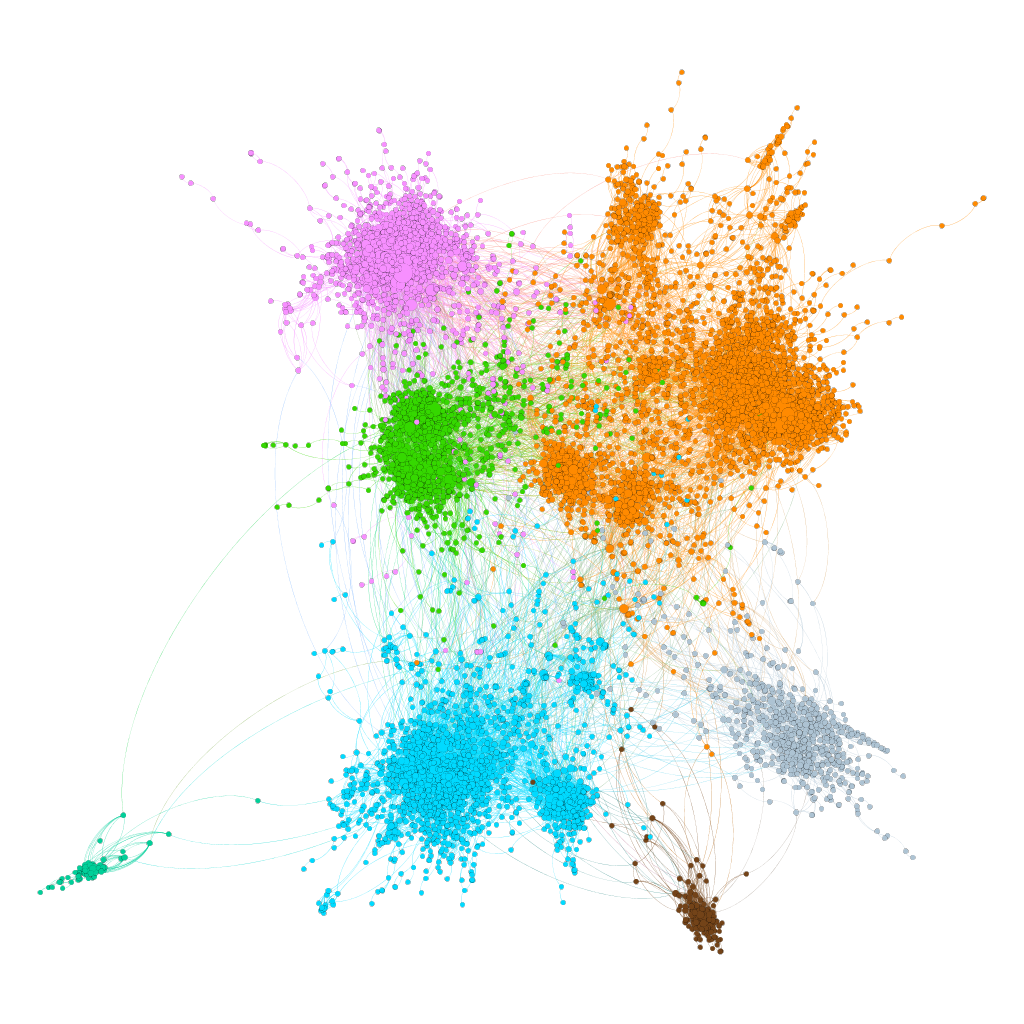
\includegraphics[width=\textwidth]{img/resultados/grado-leinen0.1.png}
%     \caption{Coeficiente 0.1.}
%   \end{subfigure}
%   \vspace{7mm}
%   \hfill
%   \begin{subfigure}[t]{0.48\textwidth}
%     \centering
%     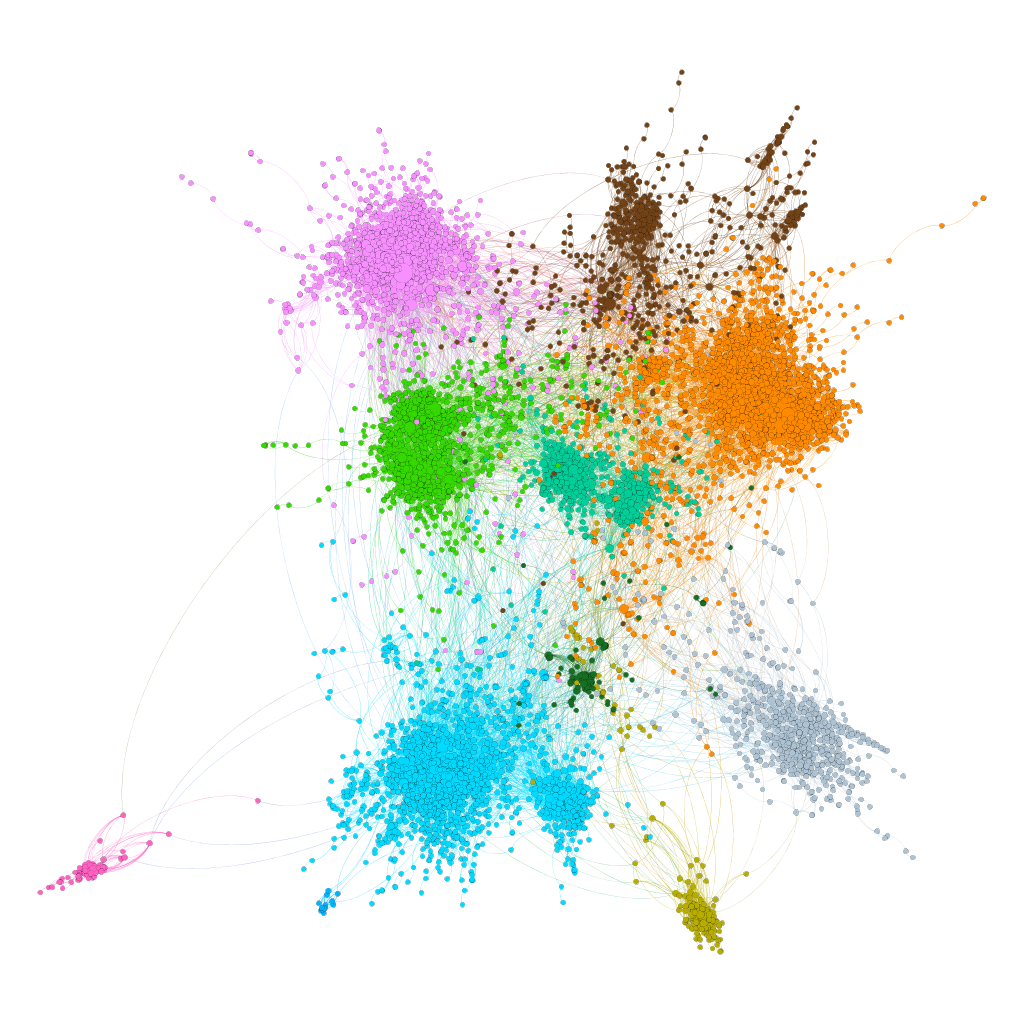
\includegraphics[width=\textwidth]{img/resultados/grado-leinen0.25.png}
%     \caption{Coeficiente 0.25.}
%   \end{subfigure}
%   \hfill
%   \begin{subfigure}[t]{0.48\textwidth}
%     \centering
%     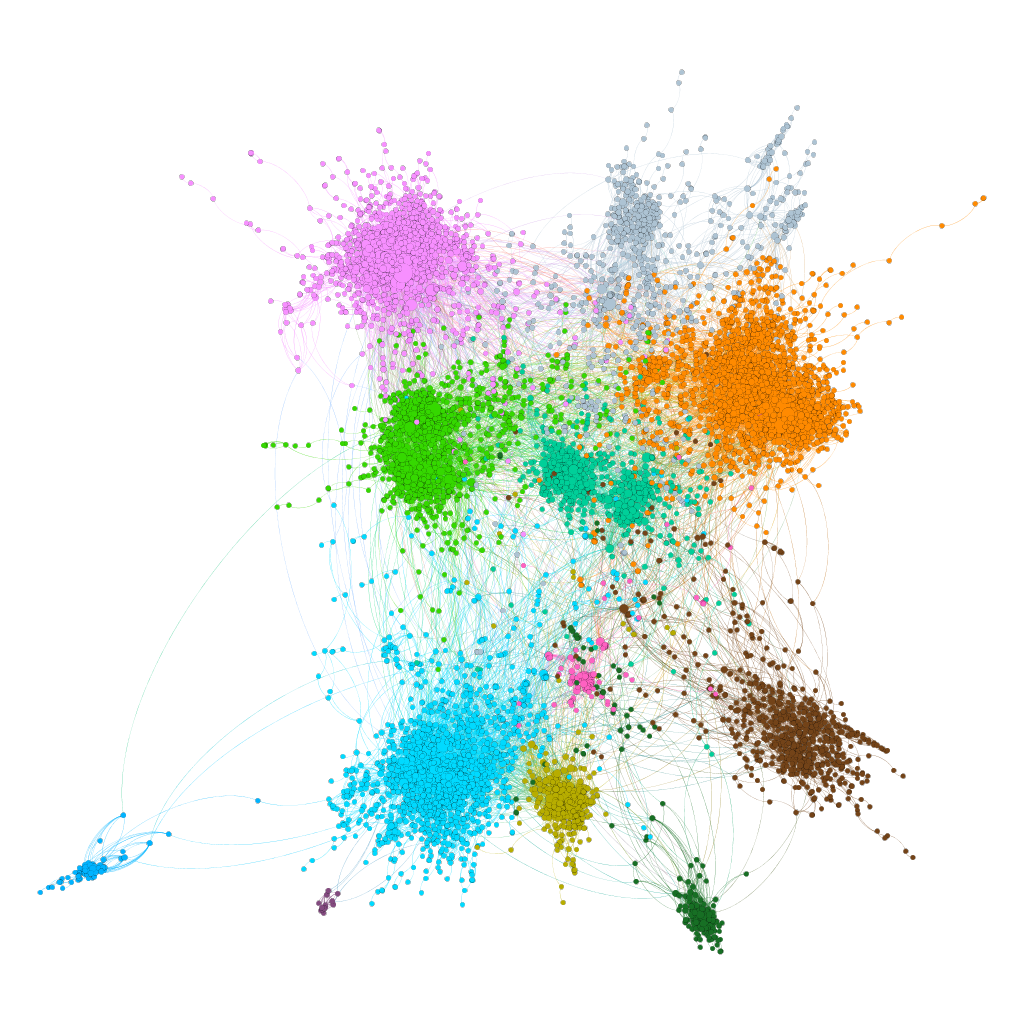
\includegraphics[width=\textwidth]{img/resultados/grado-leinen0.33.png}
%     \caption{Coeficiente 0.33.}
%   \end{subfigure}
%   \hfill
%   \begin{subfigure}[t]{0.48\textwidth}
%     \centering
%     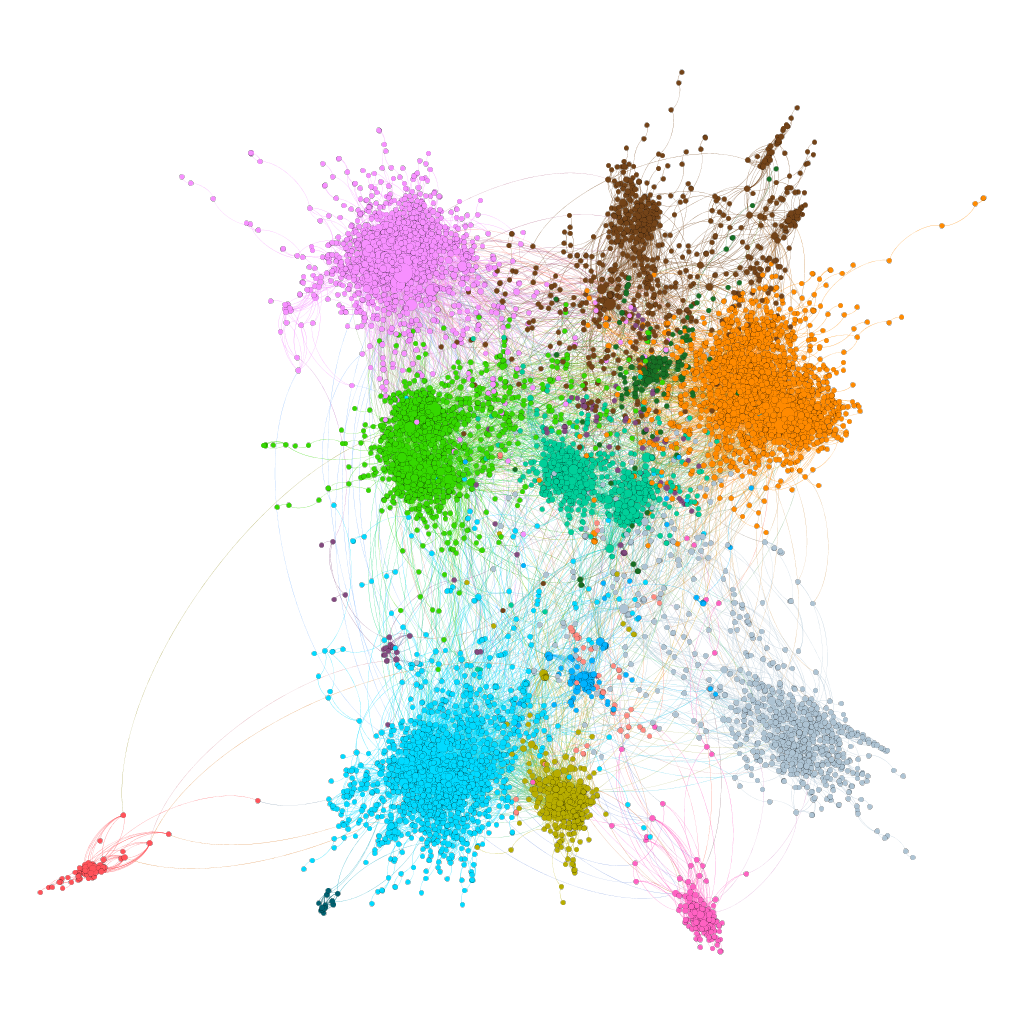
\includegraphics[width=\textwidth]{img/resultados/grado-leinen0.5.png}
%     \caption{Coeficiente 0.5.}
%   \end{subfigure}

%   \caption{Comunidades detectadas por el algoritmo Leinen para diferentes coeficientes.}
% \end{figure}

% \begin{figure}
%     \centering  
%     \begin{subfigure}[t]{0.48\textwidth}
%       \centering
%       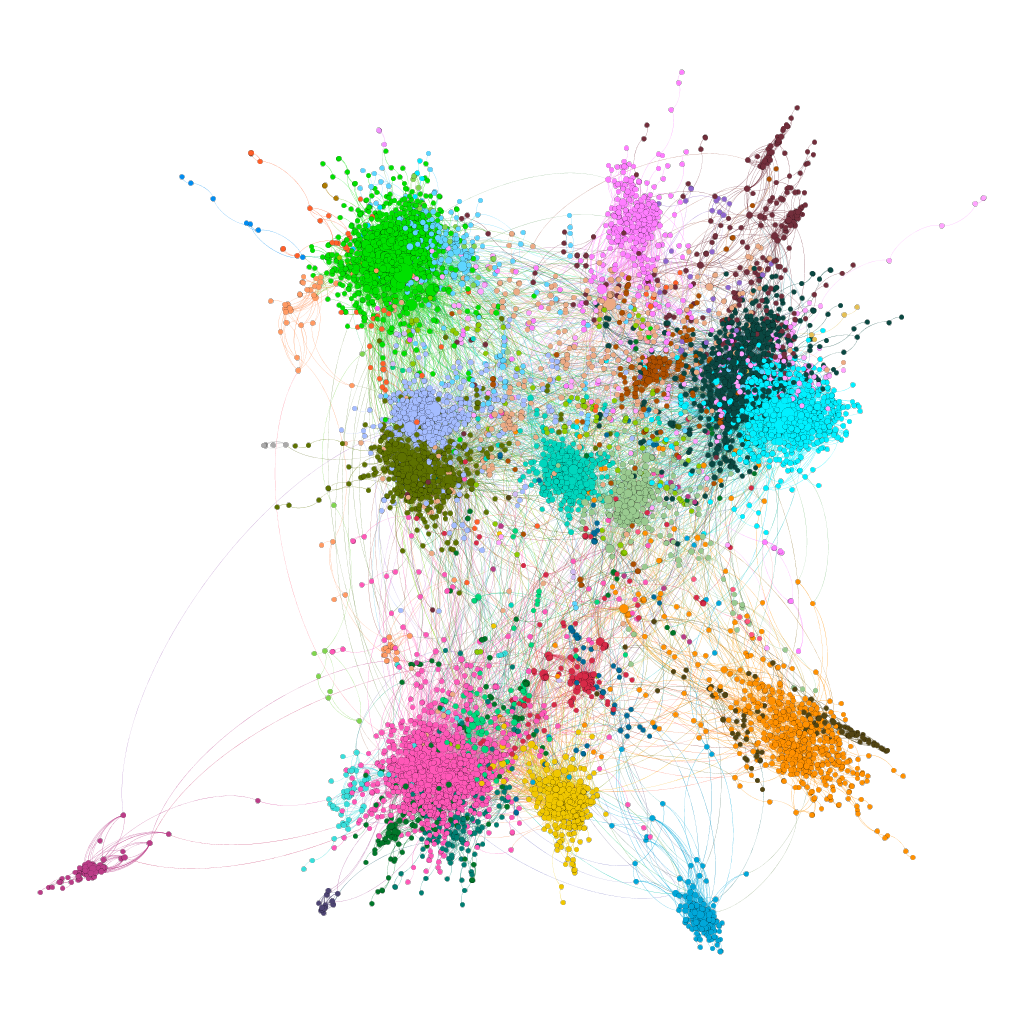
\includegraphics[width=\textwidth]{img/resultados/grado-lovaina0.5.png}
%       \caption{Coeficiente 0.5.}
%     \end{subfigure}
%     \vspace{7mm}
%     \hfill
%     \begin{subfigure}[t]{0.48\textwidth}
%       \centering
%       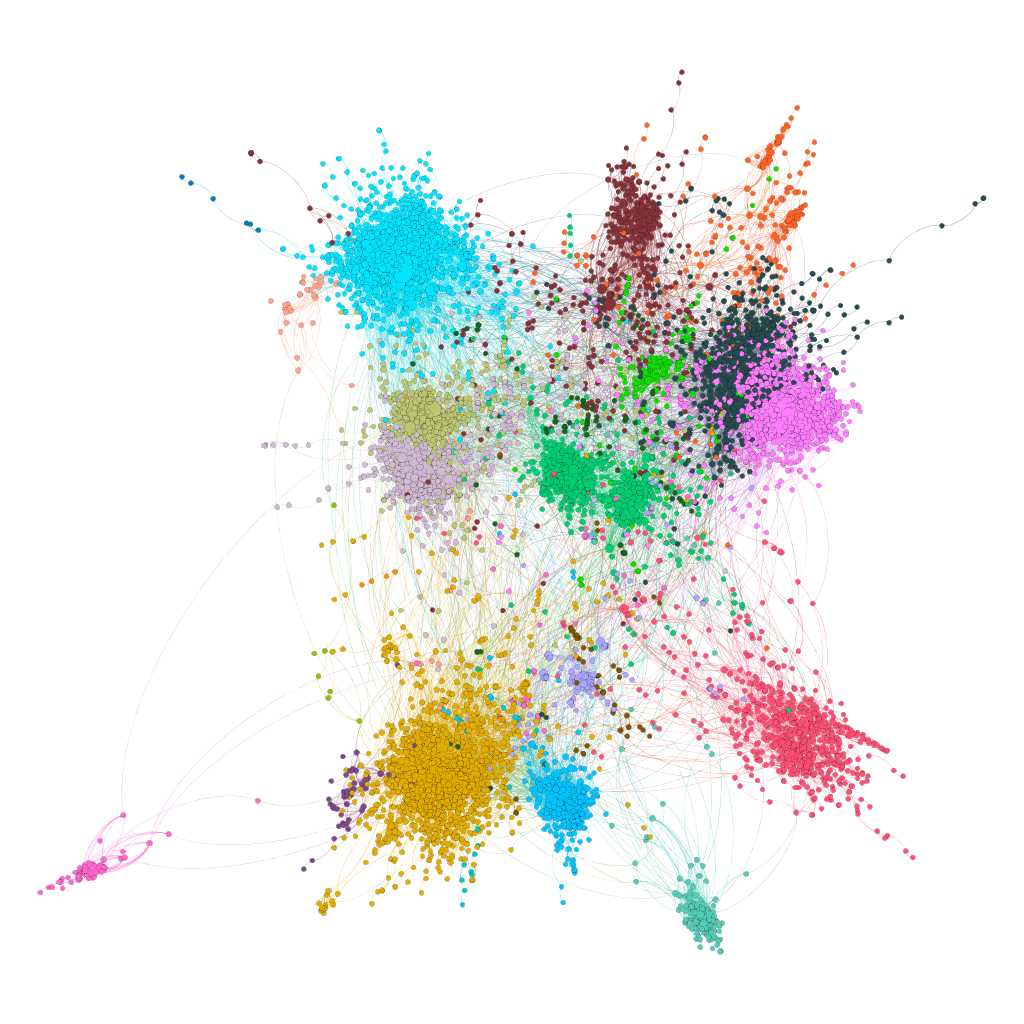
\includegraphics[width=\textwidth]{img/resultados/grado-lovaina1.png}
%       \caption{Coeficiente 1.}
%     \end{subfigure}
%     \hfill
%     \begin{subfigure}[t]{0.48\textwidth}
%       \centering
%       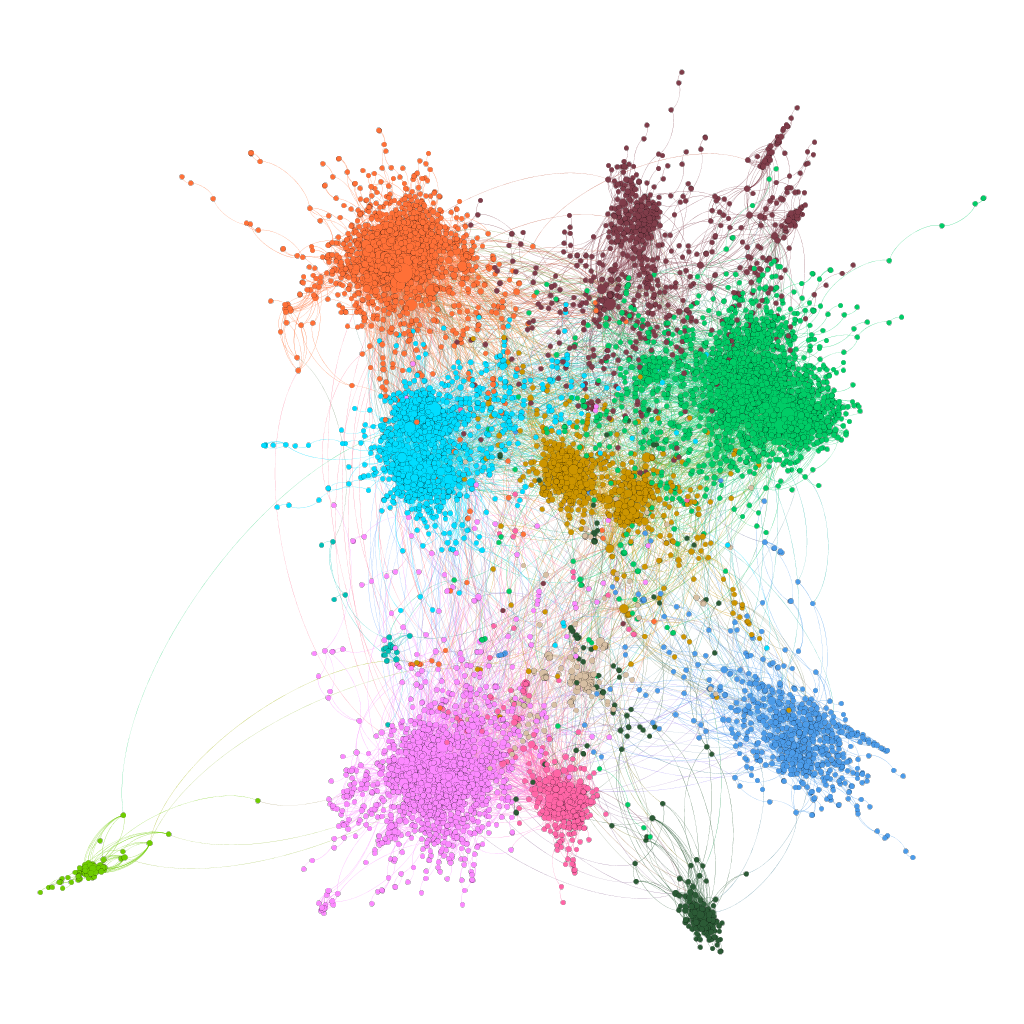
\includegraphics[width=\textwidth]{img/resultados/grado-lovaina2.png}
%       \caption{Coeficiente 2.}
%     \end{subfigure}
%     \hfill
%     \begin{subfigure}[t]{0.48\textwidth}
%       \centering
%       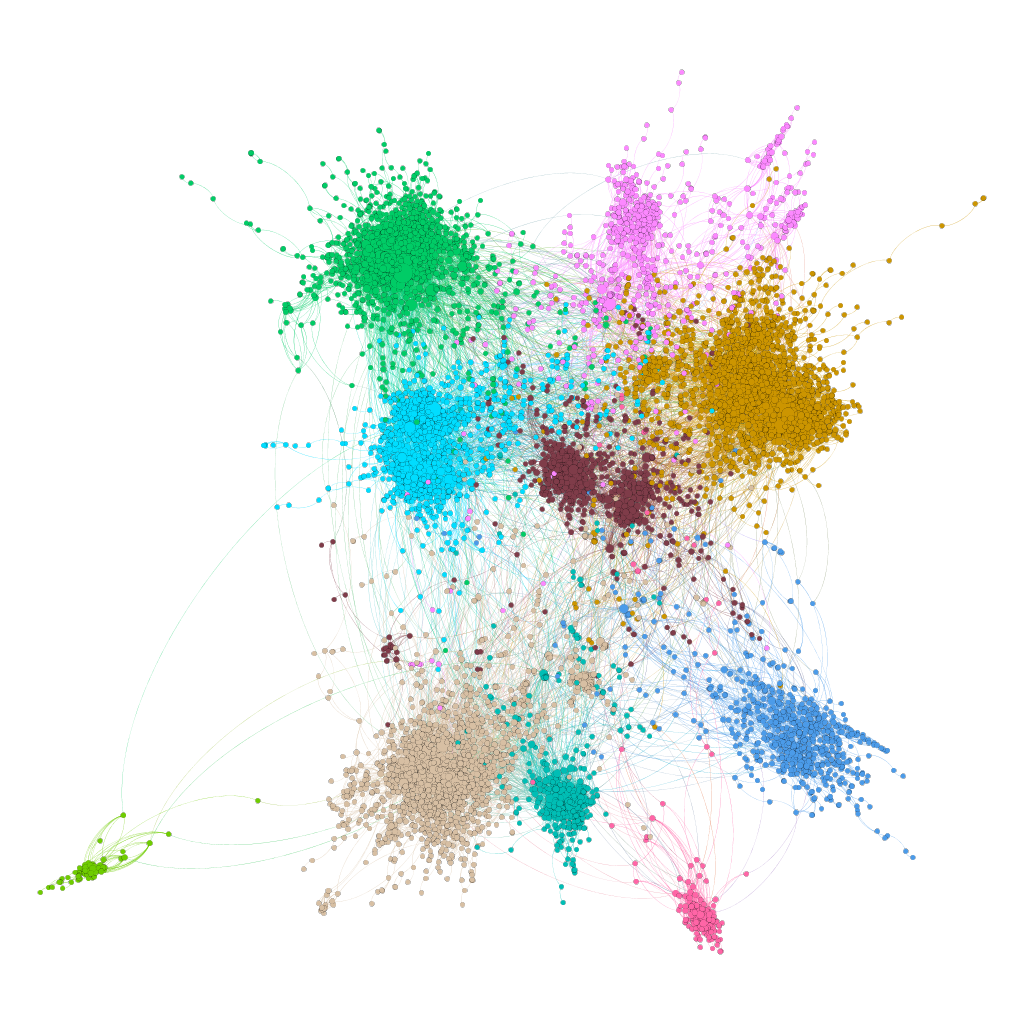
\includegraphics[width=\textwidth]{img/resultados/grado-lovaina3.png}
%       \caption{Coeficiente 3.}
%     \end{subfigure}
  
%     \caption{Comunidades detectadas por el algoritmo Lovaina para diferentes coeficientes.}
% \end{figure}

% \begin{figure}
%   \centering  
%   \begin{subfigure}[t]{0.48\textwidth}
%     \centering
%     \includegraphics[width=\textwidth]{img/resultados/lovaina0.5/communities-size-distribution.png}
%     \caption{Coeficiente 0.5.}
%   \end{subfigure}
%   \vspace{7mm}
%   \hfill
%   \begin{subfigure}[t]{0.48\textwidth}
%     \centering
%     \includegraphics[width=\textwidth]{img/resultados/lovaina1/communities-size-distribution.png}
%     \caption{Coeficiente 1.}
%   \end{subfigure}
%   \hfill
%   \begin{subfigure}[t]{0.48\textwidth}
%     \centering
%     \includegraphics[width=\textwidth]{img/resultados/lovaina2/communities-size-distribution.png}
%     \caption{Coeficiente 2.}
%   \end{subfigure}
%   \hfill
%   \begin{subfigure}[t]{0.48\textwidth}
%     \centering
%     \includegraphics[width=\textwidth]{img/resultados/lovaina3/communities-size-distribution.png}
%     \caption{Coeficiente 3.}
%   \end{subfigure}

%   \caption{Gráfico de distribuciones para el algoritmo Lovaina en diferentes coeficientes.}
% \end{figure}

% \vspace{2\baselineskip}

% \begin{figure}[H]
%   \centering
%   \resizebox{0.75\columnwidth}{!}{%
%   \begin{tabular}{| l | c || c | c |} 
%       \hline
%       \textbf{Algoritmo} & \textbf{Coeficiente} & \textbf{Modularidad} & \textbf{Clústers}  \\
%       \Xhline{2\arrayrulewidth}
%       \multirow{4}{*}{Leinen} 
%         & 0.1 & 0.941 & 7 \\ \cline{2-4}
%         & 0.25 & 0.913 & 11 \\ \cline{2-4}
%         & 0.33 & 0.901 & 11 \\ \cline{2-4}
%         & 0.5 & 0.878 & 15 \\ \cline{2-4}
%       \hline
%       \multirow{4}{*}{Lovaina} 
%         & 0.5 & 0.800 & 42 \\ \cline{2-4}
%         & 1 & 0.813 & 23 \\ \cline{2-4}
%         & 2 & 0.806 & 12 \\ \cline{2-4}
%         & 3 & 0.803 & 10 \\ \cline{2-4}
%       \hline
%   \end{tabular}
%   }
%   \caption{Modularidad y número de clústers obtenido por cada algoritmo.}
% \end{figure}